\begin{figure}[H]
    \centering
    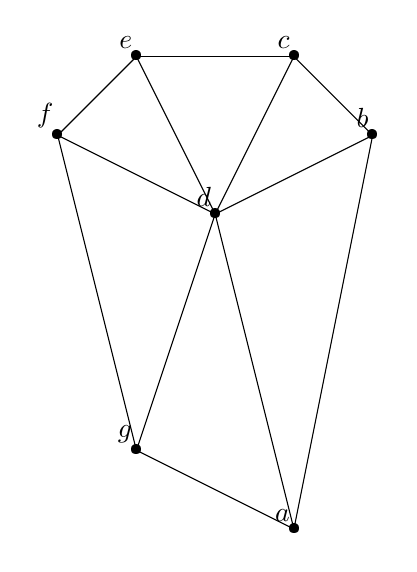
\begin{tikzpicture}
        \node[label={[label distance = -3mm]160:$a$}] at (1, -2) {\textbullet};
        \node[label={[label distance = -3mm]160:$b$}] at (2.0, 3.0) {\textbullet};
        \node[label={[label distance = -3mm]160:$c$}] at (1.0, 4) {\textbullet};
        \node[label={[label distance = -3mm]160:$d$}] at (0, 2) {\textbullet};
        \node[label={[label distance = -3mm]160:$e$}] at (-1, 4) {\textbullet};
        \node[label={[label distance = -3mm]160:$f$}] at (-2, 3) {\textbullet};
        \node[label={[label distance = -3mm]160:$g$}] at (-1, -1) {\textbullet};
        \draw (1, -2) -- (2.0, 3.0);
        \draw (0, 2) -- (2.0, 3.0);
        \draw (1.0, 4) -- (2.0, 3.0);
        \draw (1, -2) -- (0, 2);
        \draw (0, 2) -- (1.0, 4);
        \draw (-2, 3) -- (0, 2);
        \draw (-1, 4) -- (0, 2);
        \draw (-1, 4) -- (1.0, 4);
        \draw (-1, -1) -- (0, 2);
        \draw (-2, 3) -- (-1, 4);
        \draw (1, -2) -- (-1, -1);
        \draw (-1, -1) -- (-2, 3);
    \end{tikzpicture}
    \caption[Exemplo de não localidade]{Exemplo de situação em que um ponto, o ponto $d$, está
    envolvido em $O(n)$ certificados.}\label{fig:delaunay:naolocal}
\end{figure}
